\documentclass{standalone}
\usepackage{tikz}
\usetikzlibrary{patterns, positioning}
\usepackage[sfdefault]{ClearSans} %% option 'sfdefault' activates Clear Sans as the default text font
\usepackage[T1]{fontenc}

\begin{document}
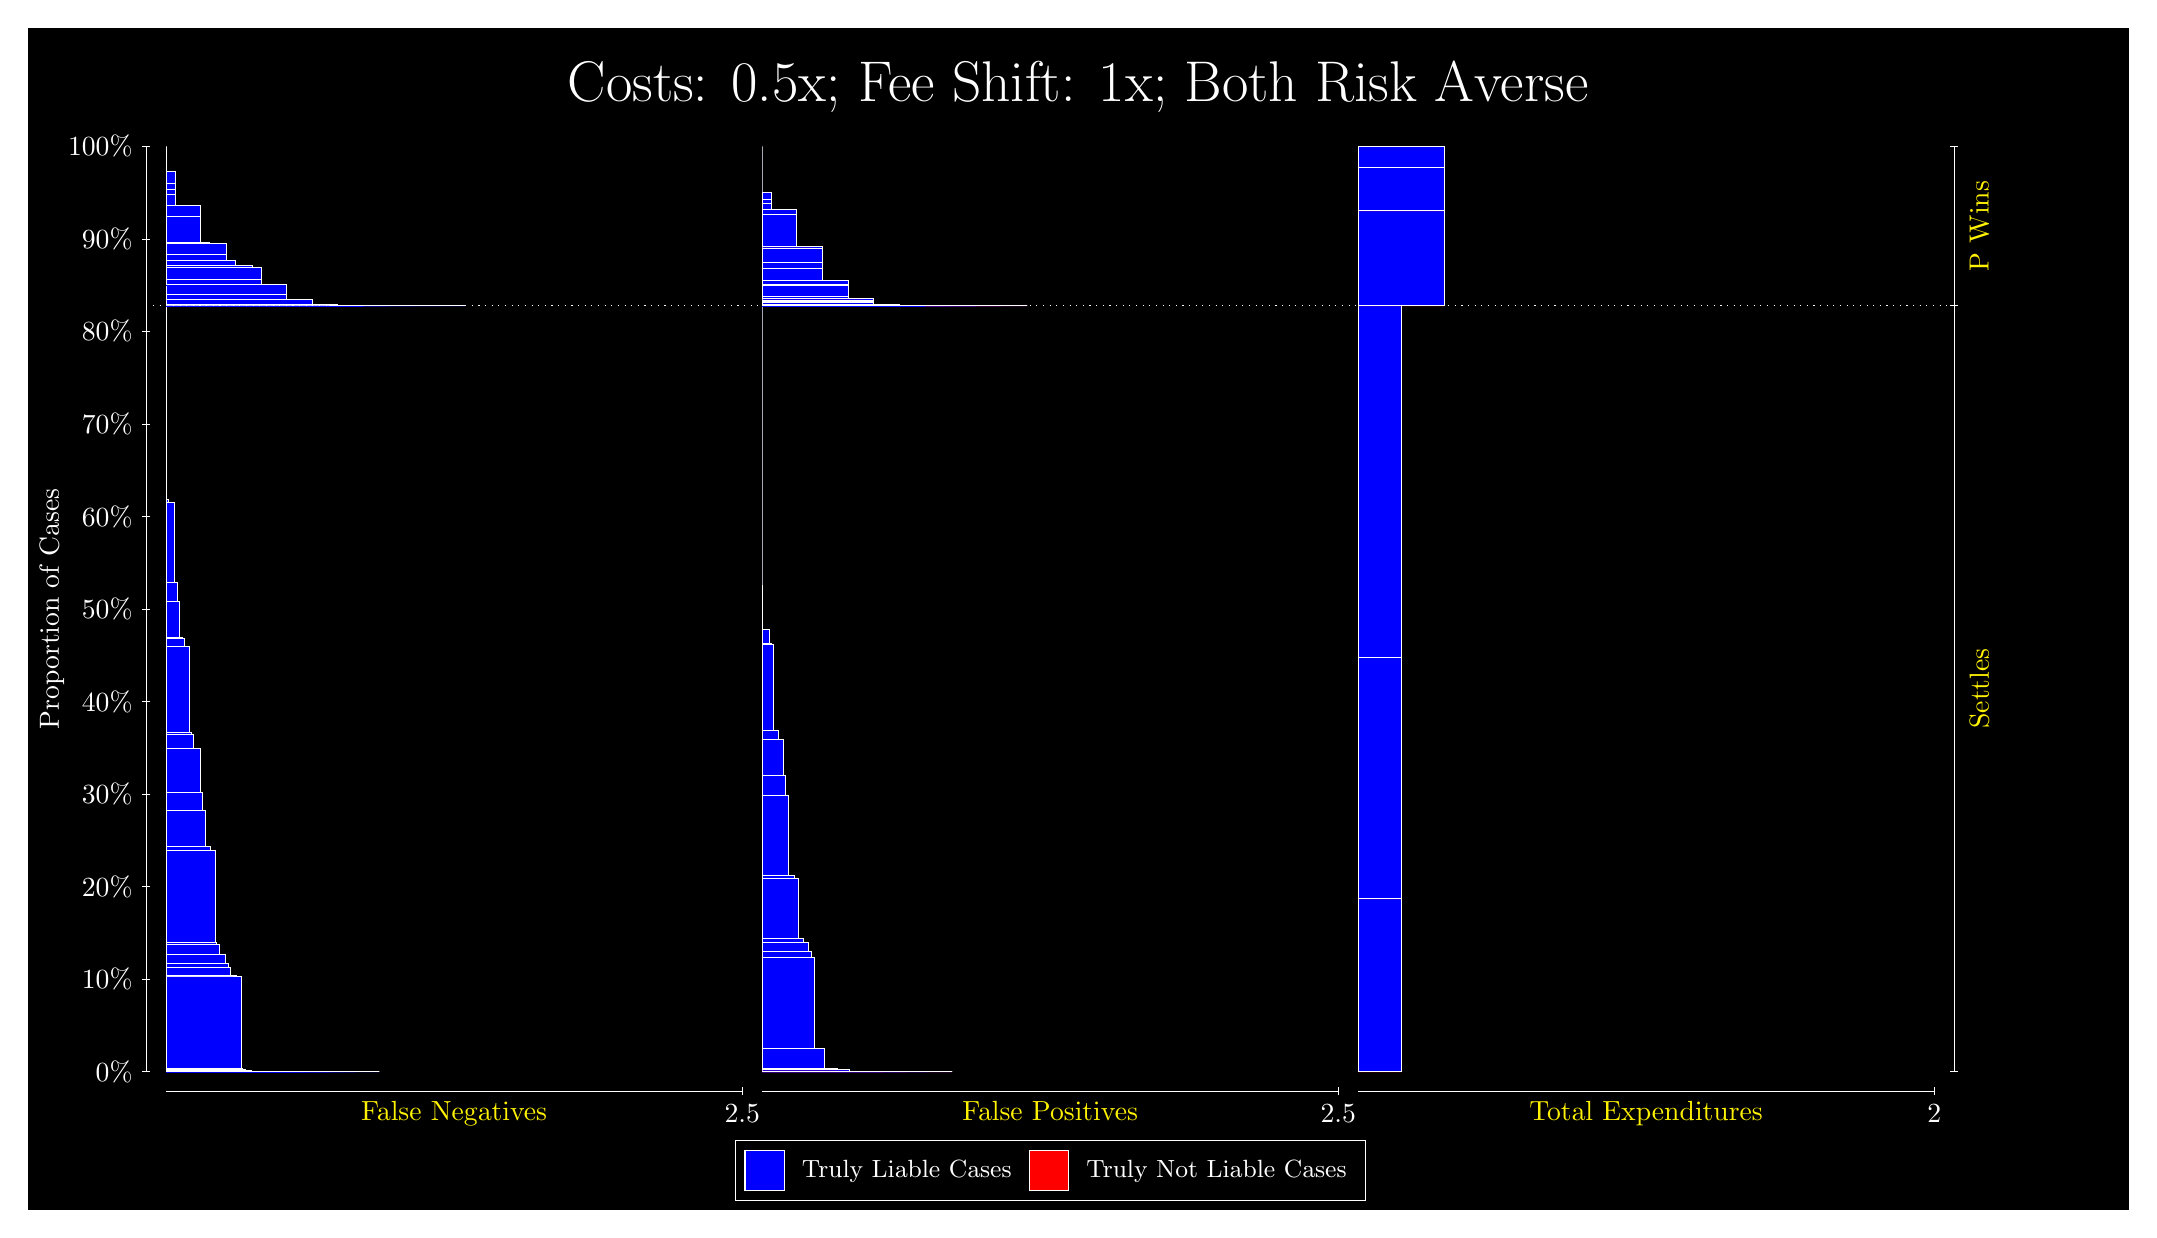
\begin{tikzpicture}
\draw[fill=black] (0,0) rectangle (26.667,15);
\draw[text=white] (0,13.5) rectangle (26.667,15) node[midway] {\huge Costs: 0.5x; Fee Shift: 1x; Both Risk Averse};
\draw[white, very thin] (1.5,1.75) -- (1.5,13.5);
\node[rotate=90, text=white, anchor=center] at (0.3, 7.625) {Proportion of Cases};
\draw[white, very thin] (1.45,1.75) -- (1.55,1.75);
\node[text=white, anchor=east] at (1.45, 1.75) {0\%};
\draw[white, very thin] (1.45,2.925) -- (1.55,2.925);
\node[text=white, anchor=east] at (1.45, 2.925) {10\%};
\draw[white, very thin] (1.45,4.1) -- (1.55,4.1);
\node[text=white, anchor=east] at (1.45, 4.1) {20\%};
\draw[white, very thin] (1.45,5.275) -- (1.55,5.275);
\node[text=white, anchor=east] at (1.45, 5.275) {30\%};
\draw[white, very thin] (1.45,6.45) -- (1.55,6.45);
\node[text=white, anchor=east] at (1.45, 6.45) {40\%};
\draw[white, very thin] (1.45,7.625) -- (1.55,7.625);
\node[text=white, anchor=east] at (1.45, 7.625) {50\%};
\draw[white, very thin] (1.45,8.8) -- (1.55,8.8);
\node[text=white, anchor=east] at (1.45, 8.8) {60\%};
\draw[white, very thin] (1.45,9.975) -- (1.55,9.975);
\node[text=white, anchor=east] at (1.45, 9.975) {70\%};
\draw[white, very thin] (1.45,11.15) -- (1.55,11.15);
\node[text=white, anchor=east] at (1.45, 11.15) {80\%};
\draw[white, very thin] (1.45,12.325) -- (1.55,12.325);
\node[text=white, anchor=east] at (1.45, 12.325) {90\%};
\draw[white, very thin] (1.45,13.5) -- (1.55,13.5);
\node[text=white, anchor=east] at (1.45, 13.5) {100\%};

\draw[white, very thin] (24.457,1.75) -- (24.457,13.5);
\draw[white, very thin] (24.407,1.75) -- (24.507,1.75);
\node[anchor=west] at (24.407, 1.75) {};
\draw[white, very thin] (24.407,11.477) -- (24.507,11.477);
\node[anchor=west] at (24.407, 11.477) {};
\draw[white, very thin] (24.407,13.5) -- (24.507,13.5);
\node[anchor=west] at (24.407, 13.5) {};

\draw[white, very thin, fill=blue] (1.75,1.75) rectangle (4.458,1.75);
\draw[white, very thin, fill=blue] (1.75,1.75) rectangle (4.1652,1.75);
\draw[white, very thin, fill=blue] (1.75,1.75) rectangle (4.1327,1.75);
\draw[white, very thin, fill=blue] (1.75,1.75) rectangle (4.0188,1.75);
\draw[white, very thin, fill=blue] (1.75,1.75) rectangle (3.8725,1.75);
\draw[white, very thin, fill=blue] (1.75,1.75) rectangle (3.8399,1.75);
\draw[white, very thin, fill=blue] (1.75,1.75) rectangle (3.8074,1.75);
\draw[white, very thin, fill=blue] (1.75,1.75) rectangle (3.7261,1.75);
\draw[white, very thin, fill=blue] (1.75,1.75) rectangle (3.6936,1.75);
\draw[white, very thin, fill=blue] (1.75,1.75) rectangle (3.5797,1.75);
\draw[white, very thin, fill=blue] (1.75,1.75) rectangle (3.5472,1.75);
\draw[white, very thin, fill=blue] (1.75,1.75) rectangle (3.5147,1.75);
\draw[white, very thin, fill=blue] (1.75,1.75) rectangle (3.4821,1.75);
\draw[white, very thin, fill=blue] (1.75,1.75) rectangle (3.4008,1.75);
\draw[white, very thin, fill=blue] (1.75,1.75) rectangle (3.3683,1.75);
\draw[white, very thin, fill=blue] (1.75,1.75) rectangle (3.287,1.75);
\draw[white, very thin, fill=blue] (1.75,1.75) rectangle (3.2544,1.75);
\draw[white, very thin, fill=blue] (1.75,1.75) rectangle (3.2219,1.7501);
\draw[white, very thin, fill=blue] (1.75,1.7501) rectangle (3.1894,1.7501);
\draw[white, very thin, fill=blue] (1.75,1.7501) rectangle (3.1568,1.7501);
\draw[white, very thin, fill=blue] (1.75,1.7501) rectangle (3.0755,1.7506);
\draw[white, very thin, fill=blue] (1.75,1.7506) rectangle (3.043,1.7506);
\draw[white, very thin, fill=blue] (1.75,1.7506) rectangle (2.9617,1.7509);
\draw[white, very thin, fill=blue] (1.75,1.7509) rectangle (2.9292,1.7509);
\draw[white, very thin, fill=blue] (1.75,1.7509) rectangle (2.8966,1.7561);
\draw[white, very thin, fill=blue] (1.75,1.7561) rectangle (2.8641,1.7583);
\draw[white, very thin, fill=blue] (1.75,1.7583) rectangle (2.8316,1.7636);
\draw[white, very thin, fill=blue] (1.75,1.7636) rectangle (2.7502,1.7825);
\draw[white, very thin, fill=blue] (1.75,1.7825) rectangle (2.7177,1.7853);
\draw[white, very thin, fill=blue] (1.75,1.7853) rectangle (2.7015,2.9599);
\draw[white, very thin, fill=blue] (1.75,2.9599) rectangle (2.6364,2.9668);
\draw[white, very thin, fill=blue] (1.75,2.9668) rectangle (2.6039,2.9669);
\draw[white, very thin, fill=blue] (1.75,2.9669) rectangle (2.5713,3.0743);
\draw[white, very thin, fill=blue] (1.75,3.0743) rectangle (2.5388,3.1234);
\draw[white, very thin, fill=blue] (1.75,3.1234) rectangle (2.5063,3.2351);
\draw[white, very thin, fill=blue] (1.75,3.2351) rectangle (2.425,3.3711);
\draw[white, very thin, fill=blue] (1.75,3.3711) rectangle (2.3924,3.3901);
\draw[white, very thin, fill=blue] (1.75,3.3901) rectangle (2.3762,4.557);
\draw[white, very thin, fill=blue] (1.75,4.557) rectangle (2.3111,4.6111);
\draw[white, very thin, fill=blue] (1.75,4.6111) rectangle (2.2786,4.6134);
\draw[white, very thin, fill=blue] (1.75,4.6134) rectangle (2.2461,5.0719);
\draw[white, very thin, fill=blue] (1.75,5.0719) rectangle (2.2135,5.2982);
\draw[white, very thin, fill=blue] (1.75,5.2982) rectangle (2.181,5.8569);
\draw[white, very thin, fill=blue] (1.75,5.8569) rectangle (2.0997,6.0343);
\draw[white, very thin, fill=blue] (1.75,6.0343) rectangle (2.0672,6.0563);
\draw[white, very thin, fill=blue] (1.75,6.0563) rectangle (2.0509,7.1455);
\draw[white, very thin, fill=blue] (1.75,7.1455) rectangle (1.9858,7.2551);
\draw[white, very thin, fill=blue] (1.75,7.2551) rectangle (1.9533,7.2603);
\draw[white, very thin, fill=blue] (1.75,7.2603) rectangle (1.9208,7.719);
\draw[white, very thin, fill=blue] (1.75,7.719) rectangle (1.8882,7.9655);
\draw[white, very thin, fill=blue] (1.75,7.9655) rectangle (1.8557,8.9783);
\draw[white, very thin, fill=blue] (1.75,8.9783) rectangle (1.7744,9.0228);
\draw[white, very thin, fill=red] (1.75,9.0228) rectangle (1.75,9.0228);
\draw[white, very thin, fill=blue] (1.75,9.0228) rectangle (1.75,11.477);
\draw[white, very thin, fill=blue] (1.75,11.477) rectangle (5.5558,11.477);
\draw[white, very thin, fill=blue] (1.75,11.477) rectangle (5.2305,11.477);
\draw[white, very thin, fill=blue] (1.75,11.477) rectangle (4.9052,11.477);
\draw[white, very thin, fill=blue] (1.75,11.477) rectangle (4.58,11.477);
\draw[white, very thin, fill=blue] (1.75,11.477) rectangle (4.58,11.477);
\draw[white, very thin, fill=blue] (1.75,11.477) rectangle (4.4661,11.477);
\draw[white, very thin, fill=blue] (1.75,11.477) rectangle (4.2547,11.478);
\draw[white, very thin, fill=blue] (1.75,11.478) rectangle (4.2547,11.478);
\draw[white, very thin, fill=blue] (1.75,11.478) rectangle (4.1408,11.478);
\draw[white, very thin, fill=blue] (1.75,11.478) rectangle (3.9294,11.49);
\draw[white, very thin, fill=blue] (1.75,11.49) rectangle (3.8155,11.49);
\draw[white, very thin, fill=blue] (1.75,11.49) rectangle (3.8155,11.49);
\draw[white, very thin, fill=blue] (1.75,11.49) rectangle (3.6041,11.553);
\draw[white, very thin, fill=blue] (1.75,11.553) rectangle (3.4903,11.553);
\draw[white, very thin, fill=blue] (1.75,11.553) rectangle (3.2788,11.615);
\draw[white, very thin, fill=blue] (1.75,11.615) rectangle (3.2788,11.743);
\draw[white, very thin, fill=blue] (1.75,11.743) rectangle (3.165,11.744);
\draw[white, very thin, fill=blue] (1.75,11.744) rectangle (3.165,11.744);
\draw[white, very thin, fill=blue] (1.75,11.744) rectangle (2.9535,11.81);
\draw[white, very thin, fill=blue] (1.75,11.81) rectangle (2.9535,11.963);
\draw[white, very thin, fill=blue] (1.75,11.963) rectangle (2.8397,11.991);
\draw[white, very thin, fill=blue] (1.75,11.991) rectangle (2.6283,12.057);
\draw[white, very thin, fill=blue] (1.75,12.057) rectangle (2.5144,12.128);
\draw[white, very thin, fill=blue] (1.75,12.128) rectangle (2.5144,12.271);
\draw[white, very thin, fill=blue] (1.75,12.271) rectangle (2.303,12.276);
\draw[white, very thin, fill=blue] (1.75,12.276) rectangle (2.1891,12.615);
\draw[white, very thin, fill=blue] (1.75,12.615) rectangle (2.1891,12.75);
\draw[white, very thin, fill=blue] (1.75,12.75) rectangle (1.9777,12.75);
\draw[white, very thin, fill=blue] (1.75,12.75) rectangle (1.8638,12.886);
\draw[white, very thin, fill=blue] (1.75,12.886) rectangle (1.8638,12.95);
\draw[white, very thin, fill=blue] (1.75,12.95) rectangle (1.8638,13.025);
\draw[white, very thin, fill=blue] (1.75,13.025) rectangle (1.8638,13.181);
\draw[white, very thin, fill=red] (1.75,13.181) rectangle (1.75,13.181);
\draw[white, very thin, fill=blue] (1.75,13.181) rectangle (1.75,13.5);
\draw[white, very thin, fill=red] (9.3189,1.75) rectangle (11.734,1.75);
\draw[white, very thin, fill=blue] (9.3189,1.75) rectangle (11.734,1.75);
\draw[white, very thin, fill=blue] (9.3189,1.75) rectangle (11.409,1.75);
\draw[white, very thin, fill=red] (9.3189,1.75) rectangle (11.149,1.75);
\draw[white, very thin, fill=blue] (9.3189,1.75) rectangle (11.149,1.75);
\draw[white, very thin, fill=blue] (9.3189,1.75) rectangle (11.084,1.75);
\draw[white, very thin, fill=red] (9.3189,1.75) rectangle (10.856,1.75);
\draw[white, very thin, fill=blue] (9.3189,1.75) rectangle (10.856,1.75);
\draw[white, very thin, fill=blue] (9.3189,1.75) rectangle (10.823,1.75);
\draw[white, very thin, fill=blue] (9.3189,1.75) rectangle (10.758,1.7505);
\draw[white, very thin, fill=red] (9.3189,1.7505) rectangle (10.709,1.7505);
\draw[white, very thin, fill=blue] (9.3189,1.7505) rectangle (10.709,1.7505);
\draw[white, very thin, fill=red] (9.3189,1.7505) rectangle (10.563,1.7505);
\draw[white, very thin, fill=blue] (9.3189,1.7505) rectangle (10.563,1.7506);
\draw[white, very thin, fill=blue] (9.3189,1.7506) rectangle (10.531,1.7506);
\draw[white, very thin, fill=blue] (9.3189,1.7506) rectangle (10.498,1.7507);
\draw[white, very thin, fill=blue] (9.3189,1.7507) rectangle (10.433,1.7749);
\draw[white, very thin, fill=red] (9.3189,1.7749) rectangle (10.417,1.7749);
\draw[white, very thin, fill=blue] (9.3189,1.7749) rectangle (10.417,1.7749);
\draw[white, very thin, fill=blue] (9.3189,1.7749) rectangle (10.384,1.7749);
\draw[white, very thin, fill=red] (9.3189,1.7749) rectangle (10.27,1.7749);
\draw[white, very thin, fill=blue] (9.3189,1.7749) rectangle (10.27,1.7854);
\draw[white, very thin, fill=blue] (9.3189,1.7854) rectangle (10.238,1.7913);
\draw[white, very thin, fill=blue] (9.3189,1.7913) rectangle (10.205,1.7915);
\draw[white, very thin, fill=blue] (9.3189,1.7915) rectangle (10.173,1.7961);
\draw[white, very thin, fill=blue] (9.3189,1.7961) rectangle (10.108,2.0468);
\draw[white, very thin, fill=blue] (9.3189,2.0468) rectangle (10.091,2.047);
\draw[white, very thin, fill=blue] (9.3189,2.047) rectangle (10.059,2.0492);
\draw[white, very thin, fill=red] (9.3189,2.0492) rectangle (9.9776,2.0492);
\draw[white, very thin, fill=blue] (9.3189,2.0492) rectangle (9.9776,3.2032);
\draw[white, very thin, fill=blue] (9.3189,3.2032) rectangle (9.945,3.281);
\draw[white, very thin, fill=blue] (9.3189,3.281) rectangle (9.9125,3.3897);
\draw[white, very thin, fill=blue] (9.3189,3.3897) rectangle (9.88,3.392);
\draw[white, very thin, fill=blue] (9.3189,3.392) rectangle (9.8475,3.441);
\draw[white, very thin, fill=blue] (9.3189,3.441) rectangle (9.7824,4.1991);
\draw[white, very thin, fill=blue] (9.3189,4.1991) rectangle (9.7661,4.204);
\draw[white, very thin, fill=blue] (9.3189,4.204) rectangle (9.7336,4.2485);
\draw[white, very thin, fill=blue] (9.3189,4.2485) rectangle (9.6523,5.2613);
\draw[white, very thin, fill=blue] (9.3189,5.2613) rectangle (9.6198,5.5078);
\draw[white, very thin, fill=blue] (9.3189,5.5078) rectangle (9.5872,5.9664);
\draw[white, very thin, fill=blue] (9.3189,5.9664) rectangle (9.5547,5.9717);
\draw[white, very thin, fill=blue] (9.3189,5.9717) rectangle (9.5222,6.0813);
\draw[white, very thin, fill=blue] (9.3189,6.0813) rectangle (9.4571,7.1705);
\draw[white, very thin, fill=blue] (9.3189,7.1705) rectangle (9.4408,7.1924);
\draw[white, very thin, fill=blue] (9.3189,7.1924) rectangle (9.4083,7.3698);
\draw[white, very thin, fill=blue] (9.3189,7.3698) rectangle (9.327,7.9285);
\draw[white, very thin, fill=blue] (9.3189,7.9285) rectangle (9.3189,11.477);
\draw[white, very thin, fill=red] (9.3189,11.477) rectangle (12.686,11.477);
\draw[white, very thin, fill=blue] (9.3189,11.477) rectangle (12.686,11.477);
\draw[white, very thin, fill=red] (9.3189,11.477) rectangle (12.36,11.477);
\draw[white, very thin, fill=blue] (9.3189,11.477) rectangle (12.36,11.477);
\draw[white, very thin, fill=red] (9.3189,11.477) rectangle (12.035,11.477);
\draw[white, very thin, fill=blue] (9.3189,11.477) rectangle (12.035,11.477);
\draw[white, very thin, fill=blue] (9.3189,11.477) rectangle (12.035,11.477);
\draw[white, very thin, fill=blue] (9.3189,11.477) rectangle (12.035,11.477);
\draw[white, very thin, fill=red] (9.3189,11.477) rectangle (11.71,11.477);
\draw[white, very thin, fill=blue] (9.3189,11.477) rectangle (11.71,11.477);
\draw[white, very thin, fill=blue] (9.3189,11.477) rectangle (11.71,11.477);
\draw[white, very thin, fill=red] (9.3189,11.477) rectangle (11.384,11.477);
\draw[white, very thin, fill=blue] (9.3189,11.477) rectangle (11.384,11.477);
\draw[white, very thin, fill=blue] (9.3189,11.477) rectangle (11.384,11.478);
\draw[white, very thin, fill=blue] (9.3189,11.478) rectangle (11.059,11.482);
\draw[white, very thin, fill=red] (9.3189,11.482) rectangle (11.059,11.482);
\draw[white, very thin, fill=blue] (9.3189,11.482) rectangle (11.059,11.484);
\draw[white, very thin, fill=blue] (9.3189,11.484) rectangle (11.059,11.492);
\draw[white, very thin, fill=blue] (9.3189,11.492) rectangle (10.734,11.517);
\draw[white, very thin, fill=blue] (9.3189,11.517) rectangle (10.734,11.532);
\draw[white, very thin, fill=red] (9.3189,11.532) rectangle (10.734,11.532);
\draw[white, very thin, fill=blue] (9.3189,11.532) rectangle (10.734,11.546);
\draw[white, very thin, fill=blue] (9.3189,11.546) rectangle (10.734,11.567);
\draw[white, very thin, fill=red] (9.3189,11.567) rectangle (10.62,11.567);
\draw[white, very thin, fill=blue] (9.3189,11.567) rectangle (10.62,11.567);
\draw[white, very thin, fill=blue] (9.3189,11.567) rectangle (10.409,11.601);
\draw[white, very thin, fill=red] (9.3189,11.601) rectangle (10.409,11.601);
\draw[white, very thin, fill=blue] (9.3189,11.601) rectangle (10.409,11.738);
\draw[white, very thin, fill=blue] (9.3189,11.738) rectangle (10.409,11.749);
\draw[white, very thin, fill=blue] (9.3189,11.749) rectangle (10.409,11.796);
\draw[white, very thin, fill=red] (9.3189,11.796) rectangle (10.295,11.796);
\draw[white, very thin, fill=blue] (9.3189,11.796) rectangle (10.295,11.796);
\draw[white, very thin, fill=blue] (9.3189,11.796) rectangle (10.083,11.949);
\draw[white, very thin, fill=blue] (9.3189,11.949) rectangle (10.083,12.033);
\draw[white, very thin, fill=blue] (9.3189,12.033) rectangle (10.083,12.209);
\draw[white, very thin, fill=blue] (9.3189,12.209) rectangle (10.083,12.227);
\draw[white, very thin, fill=red] (9.3189,12.227) rectangle (9.9694,12.227);
\draw[white, very thin, fill=blue] (9.3189,12.227) rectangle (9.9694,12.227);
\draw[white, very thin, fill=blue] (9.3189,12.227) rectangle (9.758,12.632);
\draw[white, very thin, fill=blue] (9.3189,12.632) rectangle (9.758,12.698);
\draw[white, very thin, fill=blue] (9.3189,12.698) rectangle (9.758,12.701);
\draw[white, very thin, fill=red] (9.3189,12.701) rectangle (9.6442,12.701);
\draw[white, very thin, fill=blue] (9.3189,12.701) rectangle (9.6442,12.706);
\draw[white, very thin, fill=blue] (9.3189,12.706) rectangle (9.4327,12.78);
\draw[white, very thin, fill=blue] (9.3189,12.78) rectangle (9.4327,12.833);
\draw[white, very thin, fill=blue] (9.3189,12.833) rectangle (9.4327,12.92);
\draw[white, very thin, fill=blue] (9.3189,12.92) rectangle (9.4327,12.92);
\draw[white, very thin, fill=red] (9.3189,12.92) rectangle (9.3189,12.92);
\draw[white, very thin, fill=blue] (9.3189,12.92) rectangle (9.3189,13.5);
\draw[white, very thin, fill=red] (16.888,1.75) rectangle (17.437,1.75);
\draw[white, very thin, fill=blue] (16.888,1.75) rectangle (17.437,3.9456);
\draw[white, very thin, fill=red] (16.888,3.9456) rectangle (17.437,3.9456);
\draw[white, very thin, fill=blue] (16.888,3.9456) rectangle (17.437,7.0126);
\draw[white, very thin, fill=red] (16.888,7.0126) rectangle (17.437,7.0126);
\draw[white, very thin, fill=blue] (16.888,7.0126) rectangle (17.437,11.477);
\draw[white, very thin, fill=red] (16.888,11.477) rectangle (17.986,11.477);
\draw[white, very thin, fill=blue] (16.888,11.477) rectangle (17.986,12.682);
\draw[white, very thin, fill=red] (16.888,12.682) rectangle (17.986,12.682);
\draw[white, very thin, fill=blue] (16.888,12.682) rectangle (17.986,13.239);
\draw[white, very thin, fill=red] (16.888,13.239) rectangle (17.986,13.239);
\draw[white, very thin, fill=blue] (16.888,13.239) rectangle (17.986,13.5);
\draw[white, dotted] (1.5,11.477) -- (24.457,11.477);
\draw[white, very thin] (1.75,1.5) -- (9.0689,1.5);
\node[text=yellow, anchor=north] at (5.4094, 1.5) {False Negatives};
\draw[white, very thin] (9.0689,1.45) -- (9.0689,1.55);
\node[text=white, anchor=north] at (9.0689, 1.45) {2.5};

\draw[white, very thin] (9.3189,1.5) -- (16.638,1.5);
\node[text=yellow, anchor=north] at (12.978, 1.5) {False Positives};
\draw[white, very thin] (16.638,1.45) -- (16.638,1.55);
\node[text=white, anchor=north] at (16.638, 1.45) {2.5};

\draw[white, very thin] (16.888,1.5) -- (24.207,1.5);
\node[text=yellow, anchor=north] at (20.547, 1.5) {Total Expenditures};
\draw[white, very thin] (24.207,1.45) -- (24.207,1.55);
\node[text=white, anchor=north] at (24.207, 1.45) {2};

\node[text=yellow, centered, rotate=90] at (24.777, 6.6134) {Settles};
\node[text=yellow, centered, rotate=90] at (24.777, 12.488) {P Wins};

\draw (12.978300999999998,1.5) node[draw=none] (baseCoordinate) {};
\begin{scope}[align=center]
        \matrix[scale=0.5, draw=white, below=0.5cm of baseCoordinate, nodes={draw}, column sep=0.1cm]{
            \node[rectangle, draw, minimum width=0.5cm, minimum height=0.5cm, fill=blue] {}; &
            \node[draw=none, font=\small, text=white] (B) {Truly Liable Cases}; &
            \node[rectangle, draw, minimum width=0.5cm, minimum height=0.5cm, fill=red] {}; &
            \node[draw=none, font=\small, text=white] (B) {Truly Not Liable Cases}; \\
            };
\end{scope}

\end{tikzpicture}
\end{document}